Além dos detectores de borda não-direcionais, existem detectores que se importam com qual direção está sendo feita a análise. Muitos desses operadores são baseados na noção de gradiente, que representa matematicamente exatamente essa ideia.

Dentre eles, existe o operador de Sobel \autocite{ref:sobel}, que faz o gradiente nas direções $x$ e $y$ do plano cartesiano. Em específico, considerando a operação de convolução, o filtro $h_3$ (\ref{fig:h3}) aponta na direção $-x$ (para a esquerda) e o $h_4$ (\ref{fig:h4}), na $-y$ (para cima).

\begin{figure}[H]
    \centering
    \begin{subfigure}{0.4\textwidth}
        \centering
        \begin{kmatrix}
    \matrix[square matrix]{
        -1 & 0 & 1 \\
        -2 & 0 & 2 \\
        -1 & 0 & 1 \\
    };
\end{kmatrix}
        \caption{~$h_3$}
        \label{fig:h3}
    \end{subfigure}%
    \begin{subfigure}{0.4\textwidth}
        \centering
        \begin{kmatrix}
    \matrix[square matrix]{
        -1 & -2 & -1 \\
        0 & 0 & 0 \\
        1 & 2 & 1 \\
    };
\end{kmatrix}
        \caption{~$h_4$}
        \label{fig:h4}
    \end{subfigure}

    \caption{Máscaras de Sobel.}
    \label{fig:sobel:kernel}
\end{figure}

Observando os resultados na \cref{fig:sobel}, podemos ver que quase não existe separação do corpo da borboleta com as asas na \cref{fig:sobel:y}, isso porque ela quase não apresenta variações verticais nessa região. Nessa mesma figura, no entanto, podemos ver claramente a separação do topo da asa, que não acontece na \cref{fig:sobel:x}, já que é uma região com pouca variaçao horizontal.

Além disso, podemos ver a presença do direcinamento $-x$ em vez do $+x$ na \ref{fig:sobel:x}. Em especial, na parte inferior da asa esquerda, logo abaixo do abdômen do inseto, é bem visível a borda do componente, o que não acontece na mesma região da asa direita. No tórax da borboleta também fica visível uma separação bilateral, que não é aparente na imagem original (\ref{fig:sobel:orig}).

Muitas vezes, os operadores de Sobel são combinados para extrair informações importantes do gradiente. O mais comum, é o módulo da gradiente, que no caso é encontrado por $\sqrt{\left(h_3\right)^2 + \left(h_4\right)^2}$. Ele serve como um bom detector de borda, medindo o quão forte é a variação em cada região da imagem. O resultado pode ser visto na \cref{fig:sobel:abs}.

\begin{figure}[H]
    \centering
    \begin{subfigure}{0.48\textwidth}
        \centering
        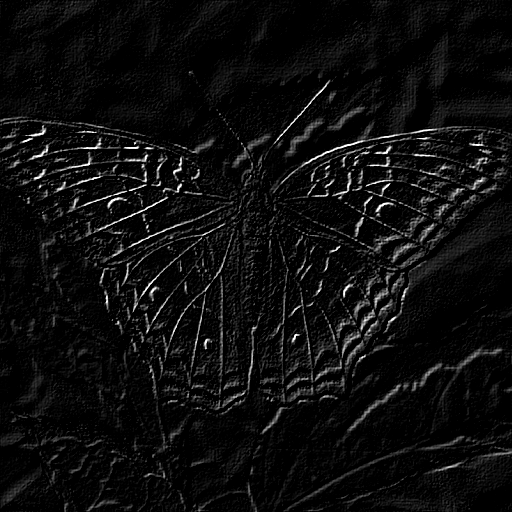
\includegraphics[width=0.9\textwidth]{imagens/butterfly.png}
        \caption{Original: \texttt{butterfly.png}.}
        \label{fig:sobel:orig}
    \end{subfigure}%
    \begin{subfigure}{0.48\textwidth}
        \centering
        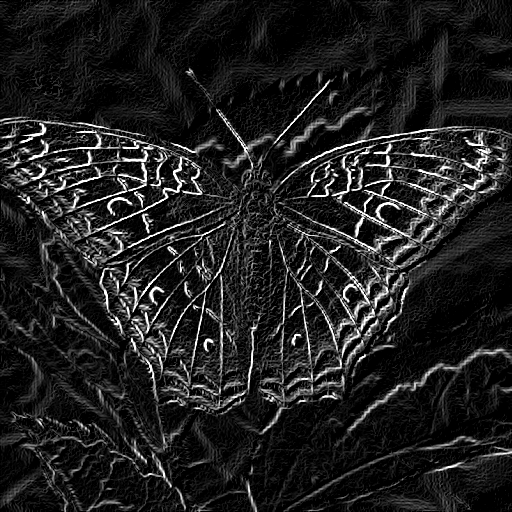
\includegraphics[width=0.9\textwidth]{resultados/butterfly_h3h4.png}
        \caption{Convolução com $h_3$ e $h_4$.}
        \label{fig:sobel:abs}
    \end{subfigure}\\[8pt]
    \begin{subfigure}{0.48\textwidth}
        \centering
        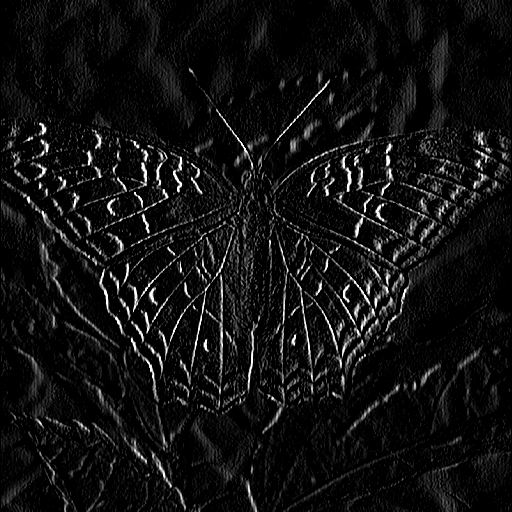
\includegraphics[width=0.9\textwidth]{resultados/butterfly_h3.png}
        \caption{Convolução com $h_3$.}
        \label{fig:sobel:x}
    \end{subfigure}%
    \begin{subfigure}{0.48\textwidth}
        \centering
        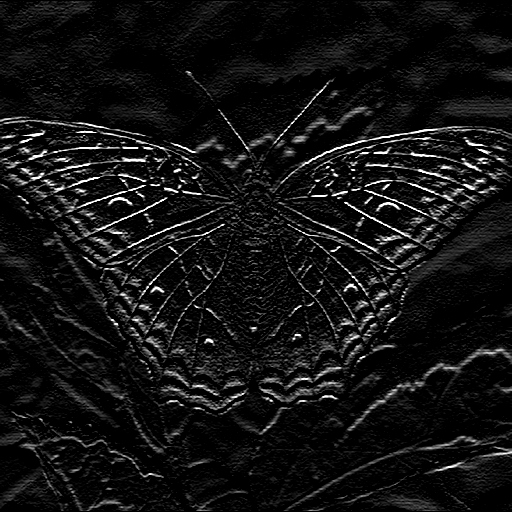
\includegraphics[width=0.9\textwidth]{resultados/butterfly_h4.png}
        \caption{Convolução com $h_4$.}
        \label{fig:sobel:y}
    \end{subfigure}

    \caption{Aplicação dos operadores de Sobel.}
    \label{fig:sobel}
\end{figure}

A aplicação do operador de Sobel, na forma mais completa, pode ser feita no programa por:

\begin{minted}{bash}
    $ python3 main.py imagens/butterfly.png h3 h4
\end{minted}
